% !TEX root = monografia.tex
\chapter{Redes Neurais Convolucionais}
\label{cap:modelo}

O nosso modelo será uma Rede Neural Convolucional com duas cabeças: uma que nos dá a distribuição $\pi(\cdot | S)$ e a outra nos dá a estimativa do valor $\hat{v}$.

\section{Os componentes da rede}

\subsection{Redes Neurais Convolucionais}

A entrada deve ser codificada como um cubo $(H, W, L)$.
A camada é codificada como um conjunto de $F$ \textit{filtros}, cada um com dimensão $(H', W', L)$.
A saída de cada filtro será uma matriz quadrada, e a saída da camada é a composição das $F$ matrizes como um cubo.
A saída do filtro é calculada passando o filtro na imagem original, produzindo o produto escalar do filtro e da seção da entrada.

\begin{figure}[h!]
\centering
    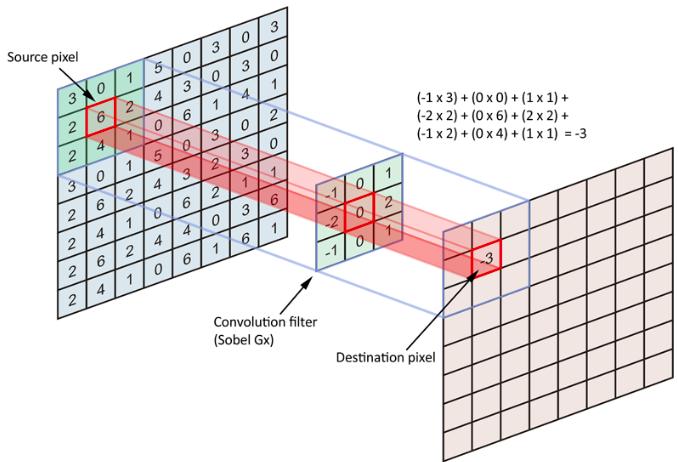
\includegraphics[width=10cm]{figuras/convolution.png}
    \caption{A operação de convolução}
    \label{fig:convolution}
\end{figure}

\subsection{ReLU}

Há algumas opções de função de ativação para redes neurais como a função sigmóide, tangente hiperbólica e a unidade linear retificada (ReLU, de \textit{Rectified Linear Unit}). A função ReLU é definida por ReLU(x) = $max(0, x)$. O ReLU, apesar de muito simples, é suficiente para as garantias de representabilidade de Redes Neurais que o utilizam e apresenta uma importante vantagem comparado com as outras funções mencionadas: ele não admite derivadas pequenas, que atrasam o processo de aprendizado. Por outro lado, o ReLU possuí o problema de\textit{neurônios mortos}, pois quando seu output é 0, sua derivada também é 0 e não ocorre aprendizado.

Para combater esse problema, foi criada uma variação do ReLU chamada de Leaky ReLU, dado pela função $max(x, \alpha x)$, onde $\alpha < 1$ é um hiperparâmetro.

\begin{figure}[h!]
\centering
    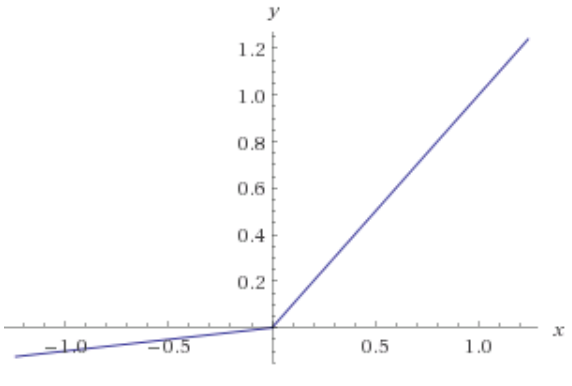
\includegraphics[width=10cm]{figuras/lrelu.png}
    \caption{O leaky ReLU}
    \label{fig:relu}
\end{figure}

\subsection{Normalização de Lote}

As camadas de Normalização de Lote (em inglês, \textit{batch normalization}) (?) são camadas normalizam sua entrada. Há uma grande quantidade de evidência empírica (?) que essas camadas aceleram o aprendizado e melhoram a performance das redes. Elas tentam combater o problema que a distribuição dos dados para as camadas internas muda durante o treinamento, pois varia de acordo com os parâmetros das camadas anteriores.